\documentclass[a4paper,12pt]{article}

% ---------- Кодировки и язык ----------
\usepackage[T2A]{fontenc}
\usepackage[utf8]{inputenc}
\usepackage[russian,english]{babel}
\usepackage{cmap}


% ---------- Геометрия ----------
\usepackage[left=2cm,right=2cm,top=2cm,bottom=2cm]{geometry}


% ---------- Графика и таблицы ----------
\usepackage{graphicx}
\usepackage{float}
\usepackage{array}
\usepackage{booktabs}
\usepackage{longtable}


% ---------- Ссылки и код ----------
\usepackage{hyperref}
\usepackage{listings}
\usepackage{xcolor}


% ---------- Прочее ----------
\usepackage{enumitem}
\usepackage{setspace}
\onehalfspacing


% ---------- Настройка листингов ----------
\definecolor{codegray}{rgb}{0.5,0.5,0.5}
\definecolor{codegreen}{rgb}{0.0,0.5,0.0}
\definecolor{backcolour}{rgb}{0.96,0.96,0.96}


\lstdefinestyle{mystyle}{
    backgroundcolor=\color{backcolour},
    commentstyle=\color{codegreen},
    keywordstyle=\color{blue},
    numberstyle=\tiny\color{codegray},
    basicstyle=\ttfamily\footnotesize,
    breakatwhitespace=false,
    breaklines=true,
    captionpos=b,
    keepspaces=true,
    numbers=left,
    numbersep=5pt,
    showspaces=false,
    showstringspaces=false,
    showtabs=false,
    tabsize=2
}
\lstset{style=mystyle}


% ---------- Гиперссылки ----------
\hypersetup{
    colorlinks=true,
    linkcolor=black,
    urlcolor=blue,
    citecolor=black
}


% =========================================================
\begin{document}


% ---------- Титульный лист ----------
\begin{titlepage}
    \centering
    {\scshape\large Министерство науки и высшего образования Российской Федерации\par}
    \vspace{0.5cm}
    {\scshape\large Университет ИТМО\par}
    \vspace{0.3cm}
    {\scshape\large Факультет программной инженерии и компьютерной техники\par}
    \vspace{3cm}


    {\Large\bfseries Мастер-класс №~3\par}
    \vspace{0.5cm}
    {\Large\bfseries «Программирование микроконтроллеров с~операционной системой (FreeRTOS)»\par}
    \vspace{1cm}
    {\large Вариант: Flappy Bird\par}


    \vspace{4cm}
    \begin{flushright}
        \begin{tabular}{rl}
            \textbf{Исполнители:} & Ясаков Артем \\
                                  & Пахомов Игнат \\[0.3cm]
            \textbf{Преподаватели:} & Быковский~С.\,В. \\
                                    & Гончаров~А.\,А. \\
        \end{tabular}
    \end{flushright}


    \vfill
    {\large Санкт-Петербург\par}
    {\large 2026\par}
\end{titlepage}


% ---------- Оглавление ----------
\tableofcontents
\newpage


% =========================================================
\section{Цель и задачи работы}


\textbf{Цель работы:} получить практические навыки разработки многозадачных программ для микроконтроллеров с~использованием операционной системы реального времени FreeRTOS, а~также освоить механизмы межзадачного взаимодействия: очереди, мьютексы и~планирование задач.


\textbf{Задачи:}
\begin{enumerate}[label=\arabic*.]
    \item Изучить архитектуру FreeRTOS: задачи, планировщик, очереди, мьютексы, семафоры.
    \item Освоить процесс создания проекта с~FreeRTOS в~среде STM32CubeIDE (CMSIS-RTOS v1).
    \item Разработать многозадачное приложение на базе FreeRTOS: разбить функциональность игры Flappy Bird на независимые задачи.
    \item Реализовать драйвер опроса клавиатуры через I2C (расширитель PCA9538) и~драйвер вывода пиксельной графики на OLED-дисплей SSD1306.
    \item Реализовать звуковое сопровождение через PWM (TIM2) на пьезо-зуммере.
    \item Реализовать игровую механику Flappy Bird: гравитацию, генерацию препятствий, детектирование столкновений, подсчёт очков.
    \item Обеспечить защиту от гонок данных с~помощью мьютексов.
    \item Протестировать программу на стенде SDK-1.1M.
\end{enumerate}


% =========================================================
\section{Схема взаимодействия процессора и периферийных устройств}


Схема взаимодействия выполнена в виде диаграммы последовательностей (PlantUML).


\begin{figure}[H]
    \centering
    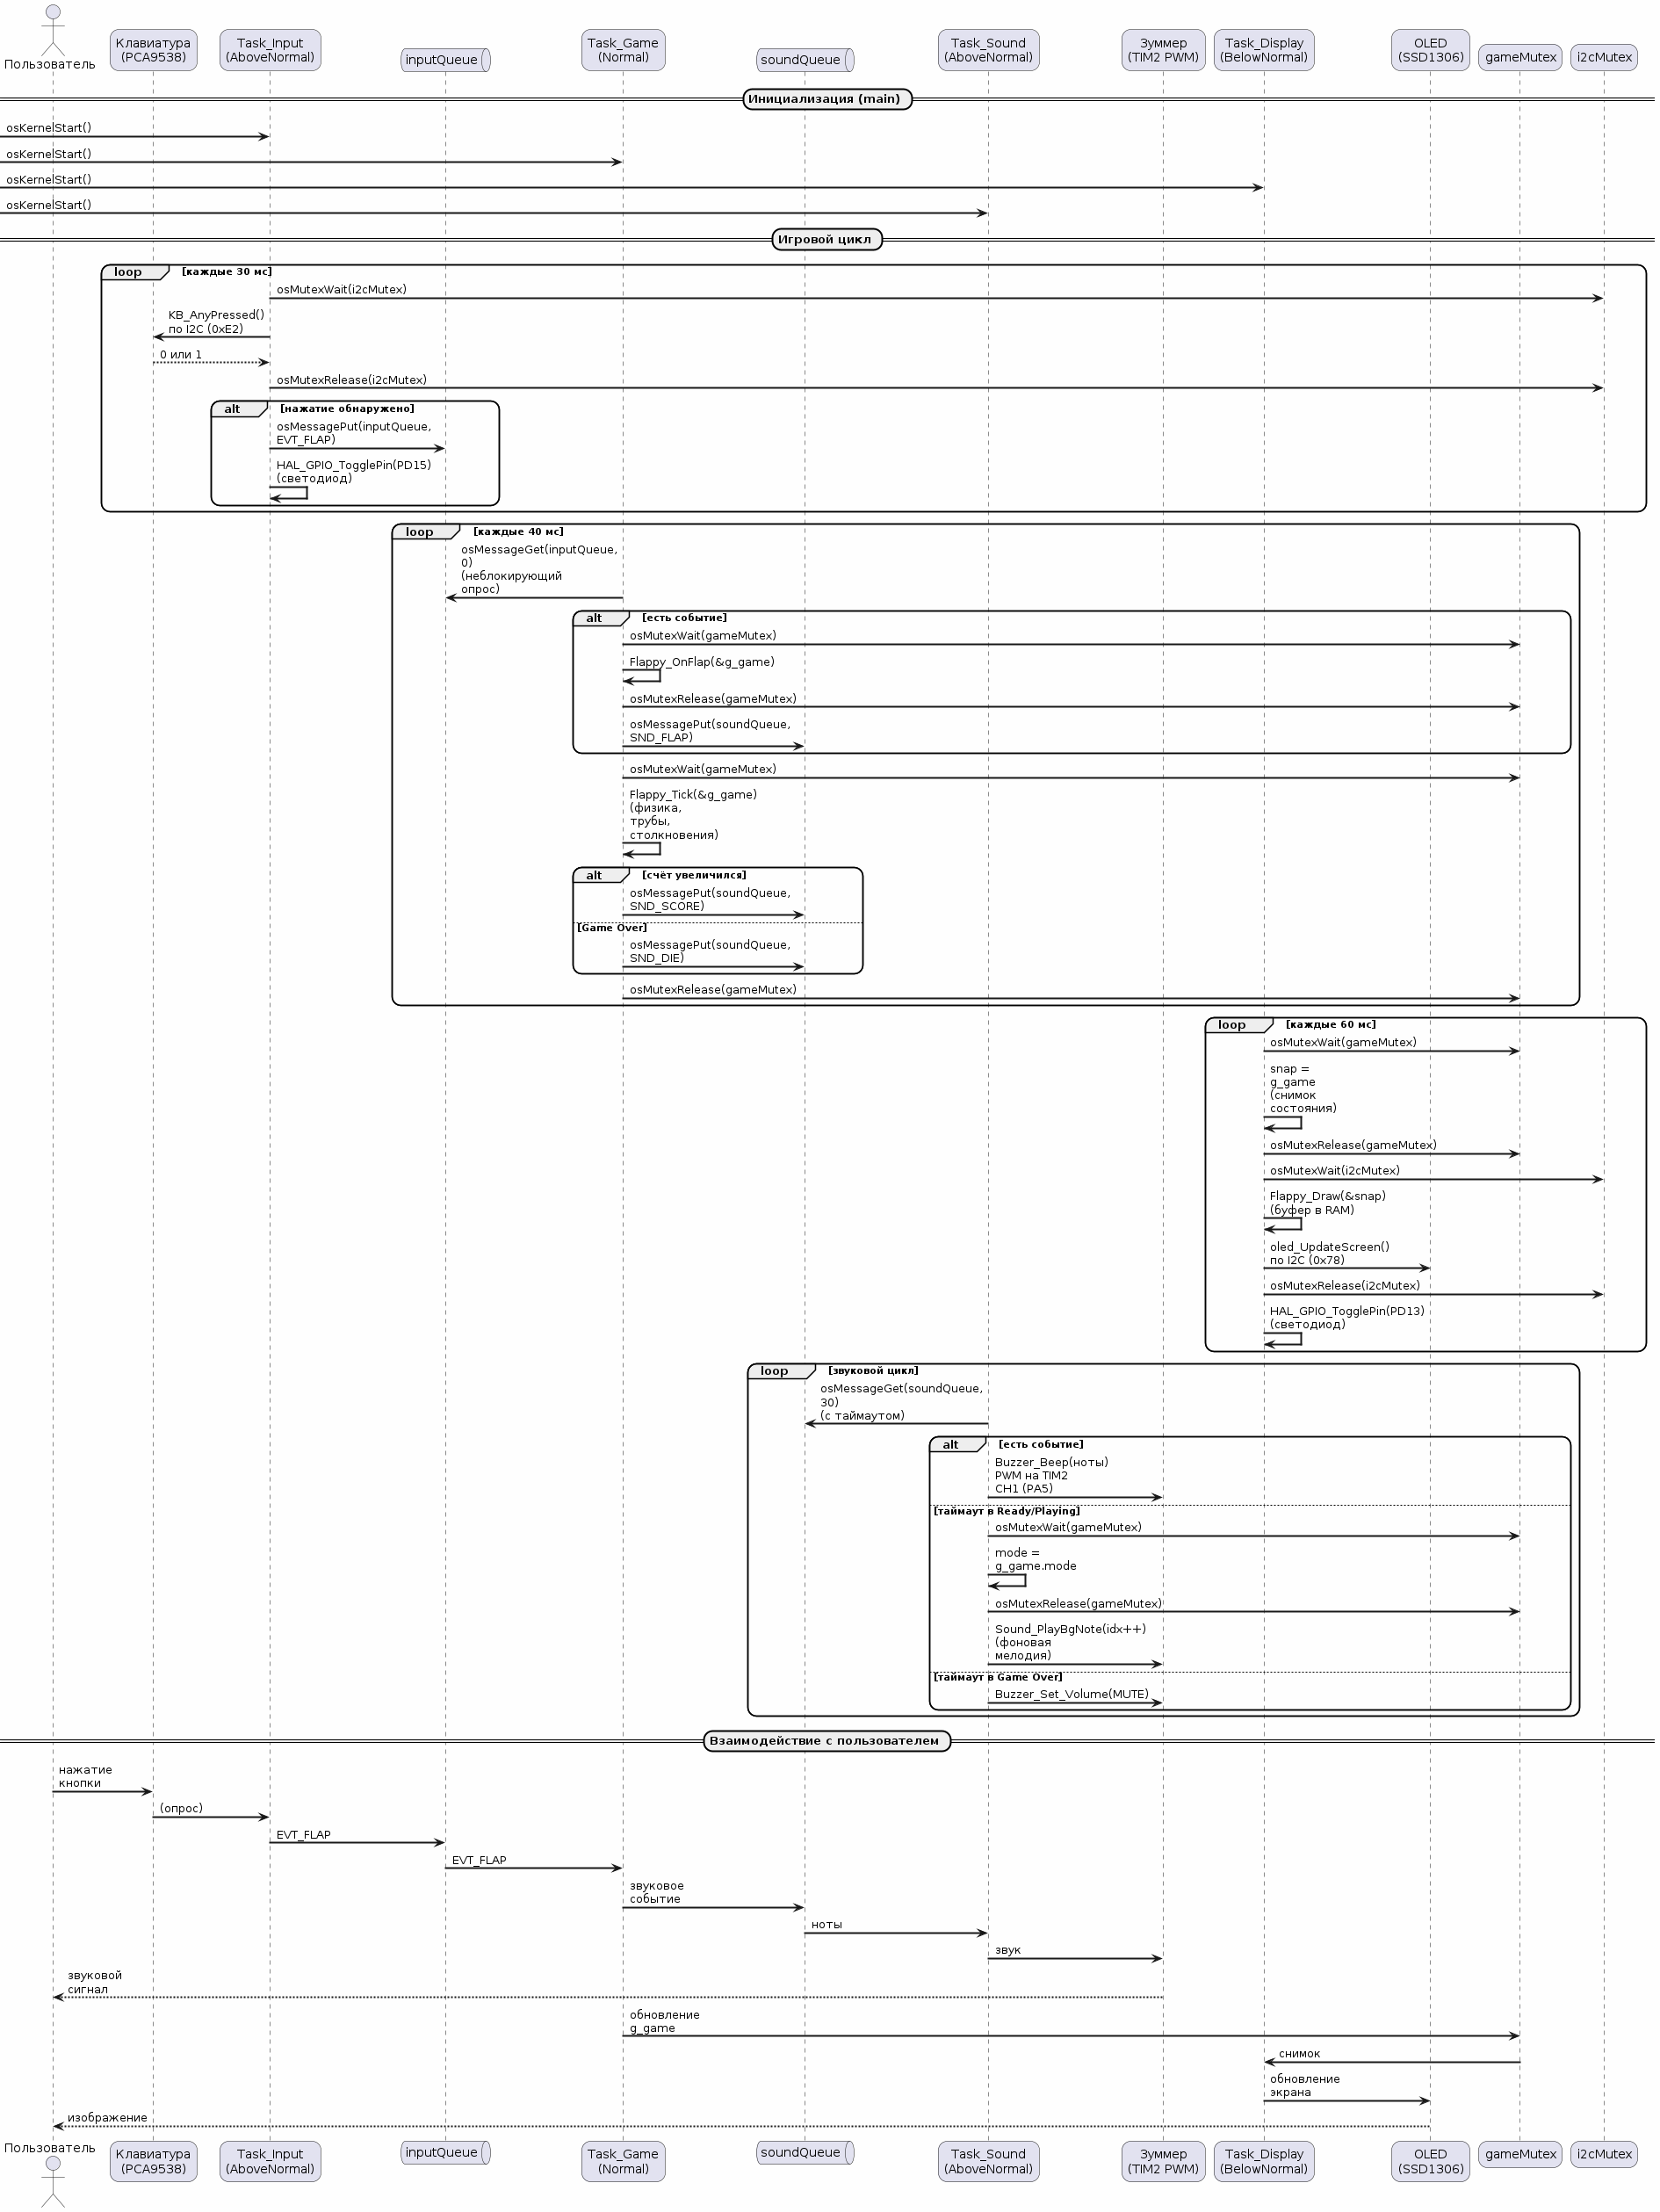
\includegraphics[width=\textwidth]{MK3_plantuml.png}
    \caption{Диаграмма последовательности взаимодействия задач FreeRTOS и периферии}
    \label{fig:sequence}
\end{figure}


% =========================================================
\section{Описание процессов, изображённых на схеме}


\subsection{Инициализация}


В функции \texttt{main()} выполняется:
\begin{itemize}
    \item \texttt{HAL\_Init()} — инициализация HAL и~SysTick;
    \item \texttt{SystemClock\_Config()} — HSE 25~МГц, PLL $\to$ SYSCLK 168~МГц, AHB~=~168~МГц, APB1~=~42~МГц, APB2~=~84~МГц;
    \item \texttt{MX\_GPIO\_Init()}, \texttt{MX\_I2C1\_Init()}, \texttt{MX\_USART1\_UART\_Init()}, \texttt{MX\_TIM2\_Init()} — настройка периферии (генерируется CubeMX);
    \item \texttt{oled\_Init()} — отправка по I2C на адрес \texttt{0x78} команд инициализации SSD1306;
    \item \texttt{Buzzer\_Init()} — инициализация ШИМ на TIM2 CH1 (PA5);
    \item \texttt{Buzzer\_BootBeep()} — два звуковых сигнала при включении;
    \item \texttt{MX\_FREERTOS\_Init()} — создание очередей, мьютексов и~задач FreeRTOS;
    \item \texttt{osKernelStart()} — запуск планировщика.
\end{itemize}


\subsection{Подсистема ввода (Task\_Input)}


Задача \texttt{Task\_Input} (приоритет AboveNormal, стек 256 байт) опрашивает клавиатуру:
\begin{itemize}
    \item Клавиатура подключена к расширителю PCA9538 (I2C-адрес \texttt{0xE2}), организована в матрицу $4\times3$.
    \item Строки — $P0..P3$ расширителя; столбцы — $P4..P6$.
    \item Функция \texttt{KB\_AnyPressed()} последовательно опрашивает все строки через \texttt{Check\_Row()} и возвращает 1 при любом нажатии.
    \item Реализован программный антидребезг: обнаружение перехода «не нажато $\to$ нажато» (переменная \texttt{prev}).
    \item При обнаружении нажатия в очередь \texttt{inputQueue} отправляется событие \texttt{EVT\_FLAP}.
    \item Индикация нажатия: светодиод PD15 переключается при каждом нажатии (\texttt{HAL\_GPIO\_TogglePin}).
    \item Доступ к шине I2C защищён мьютексом \texttt{i2cMutex}.
    \item Период опроса: 30~мс.
\end{itemize}


\subsection{Подсистема игровой логики (Task\_Game)}


Задача \texttt{Task\_Game} (приоритет Normal, стек 256 байт) содержит основной игровой цикл:
\begin{itemize}
    \item Считывает все накопившиеся события из \texttt{inputQueue} (неблокирующий \texttt{osMessageGet} с таймаутом 0).
    \item При получении \texttt{EVT\_FLAP} вызывает \texttt{Flappy\_OnFlap()}, которая в~зависимости от режима: запускает игру (Ready), задаёт скорость взмаха (Playing) или перезапускает игру (Game Over).
    \item Каждый тик (40~мс) вызывает \texttt{Flappy\_Tick()}:
        \begin{itemize}
            \item Обновляет вертикальную скорость птицы с учётом гравитации (\texttt{GRAVITY = 18});
            \item Двигает трубы влево (\texttt{PIPE\_SPEED = 2});
            \item Проверяет столкновения (\texttt{bird\_hits\_pipe}): перекрытие по X и выход за пределы зазора по Y;
            \item Проверяет выход за границы экрана (земля \texttt{GROUND\_Y = 60});
            \item При прохождении трубы увеличивает счёт и обновляет лучший результат (\texttt{best});
            \item Ушедшие за экран трубы пересоздаются справа со случайной позицией зазора.
        \end{itemize}
    \item Отправляет звуковые события в \texttt{soundQueue} при изменении игрового состояния.
    \item Доступ к состоянию игры \texttt{g\_game} защищён мьютексом \texttt{gameMutex}.
\end{itemize}


\subsubsection{Генерация препятствий}

Позиция зазора трубы вычисляется с помощью 16-битного LFSR-генератора псевдослучайных чисел:
\begin{verbatim}
lfsr ^= (lfsr << 7); lfsr ^= (lfsr >> 9); lfsr ^= (lfsr << 8);
\end{verbatim}
Зазор располагается в диапазоне $[8, \texttt{SCREEN\_H} - \texttt{PIPE\_GAP} - 10]$, что обеспечивает проходимость уровня.


\subsection{Подсистема отображения (Task\_Display)}


Задача \texttt{Task\_Display} (приоритет BelowNormal, стек 768 байт) отрисовывает игру на OLED:
\begin{itemize}
    \item Делает снимок состояния \texttt{g\_game} под мьютексом \texttt{gameMutex} и~работает с локальной копией — это исключает длительное удержание мьютекса во время отрисовки.
    \item Вызывает \texttt{Flappy\_Draw()}, которая:
        \begin{itemize}
            \item Заливает буфер чёрным цветом (\texttt{oled\_Fill(Black)});
            \item Рисует землю (сплошной прямоугольник от \texttt{GROUND\_Y} до низа экрана);
            \item Рисует трубы (верхнюю и нижнюю части для каждой из двух труб) с~помощью \texttt{fill\_rect()};
            \item Рисует птицу (квадрат $6\times6$ пикселей с глазом);
            \item Выводит счёт в правом верхнем углу;
            \item В режиме Ready выводит надписи «FLAPPY» и~«press key»;
            \item В режиме Game Over выводит «OVER» и~лучший результат.
        \end{itemize}
    \item Отправляет кадровый буфер на дисплей через \texttt{oled\_UpdateScreen()} (покадровая запись 8 страниц по I2C).
    \item Доступ к I2C защищён мьютексом \texttt{i2cMutex}.
    \item Индикация: светодиод PD13 переключается при каждой отрисовке.
    \item Период обновления: 60~мс.
\end{itemize}


\subsection{Подсистема звука (Task\_Sound)}


Задача \texttt{Task\_Sound} (приоритет AboveNormal, стек 384 байт) обеспечивает звуковое сопровождение:
\begin{itemize}
    \item Приоритетно обрабатывает события из \texttt{soundQueue} (звуковые эффекты):
        \begin{itemize}
            \item \texttt{SND\_FLAP} — две короткие ноты C6 + E6;
            \item \texttt{SND\_SCORE} — три ноты E5 $\to$ G5 $\to$ C6;
            \item \texttt{SND\_DIE} — нисходящая мелодия из 7 нот (G5 $\to$ F4 $\to$ G3);
            \item \texttt{SND\_START} — восходящее арпеджио C5 $\to$ E5 $\to$ G5 $\to$ C6.
        \end{itemize}
    \item При отсутствии событий в очереди (таймаут 30~мс) проигрывает фоновую мелодию — циклический мотив из 16 нот (C5, E5, G5, E5, C5, E5, G5, C6, A5, G5, E5, C5, D5, F5, A5, G5).
    \item В режиме Game Over зуммер отключается (\texttt{BUZZER\_VOLUME\_MUTE}).
    \item Для генерации звука используется PWM на TIM2 (Channel 1, PA5). Частота ноты задаётся через делитель \texttt{PSC}, громкость — через скважность (\texttt{CCR1}). Формула: $f = \texttt{TIMCLK} / ((\texttt{PSC}+1) \cdot (\texttt{ARR}+1))$.
\end{itemize}


\subsection{Синхронизация и защита от гонок}


\begin{itemize}
    \item \texttt{gameMutex} — мьютекс, защищающий глобальное состояние \texttt{g\_game}. Используется задачами Task\_Game, Task\_Display и~Task\_Sound при чтении/записи игрового состояния. Предотвращает ситуацию, когда одна задача модифицирует состояние в~то время, как другая его читает.
    \item \texttt{i2cMutex} — мьютекс, защищающий шину I2C1. Используется задачами Task\_Input (опрос клавиатуры) и~Task\_Display (отправка кадра на OLED). I2C не реентерабелен, поэтому требуется мьютекс для исключения одновременных транзакций.
    \item \texttt{inputQueue} — очередь сообщений (FIFO, ёмкость 8, тип \texttt{uint16\_t}) для передачи событий от Task\_Input к~Task\_Game. Обеспечивает асинхронную доставку нажатий клавиш без потерь.
    \item \texttt{soundQueue} — очередь сообщений (FIFO, ёмкость 8, тип \texttt{uint16\_t}) для передачи событий \texttt{SoundEvt\_t} от Task\_Game к~Task\_Sound. Позволяет накапливать несколько звуковых событий.
\end{itemize}


\subsection{Конфигурация FreeRTOS}


\begin{table}[H]
    \centering
    \begin{tabular}{l|l}
        \toprule
        \textbf{Параметр} & \textbf{Значение} \\
        \midrule
        Планирование & Вытесняющее с квантованием времени \\
        configMAX\_PRIORITIES & 7 \\
        configTICK\_RATE\_HZ & 1000 Гц \\
        configTOTAL\_HEAP\_SIZE & 20480 байт \\
        configMINIMAL\_STACK\_SIZE & 128 слов \\
        configUSE\_MUTEXES & 1 \\
        configUSE\_PREEMPTION & 1 \\
        configUSE\_TIME\_SLICING & 1 \\
        configGENERATE\_RUN\_TIME\_STATS & 1 \\
        \bottomrule
    \end{tabular}
    \caption{Параметры FreeRTOSConfig.h}
\end{table}


% =========================================================
\section{Руководство пользователя}


\subsection{Подключение стенда}
\begin{enumerate}
    \item Подключить USB-кабель в разъём \texttt{DBG USB} стенда SDK-1.1M.
    \item Убедиться, что загорелся светодиод \texttt{VTGT}.
    \item В Linux проверить порты: \texttt{ls /dev/ttyUSB*} — должны появиться \texttt{ttyUSB1} и~\texttt{ttyUSB2}.
\end{enumerate}


\subsection{Загрузка программы}
\begin{enumerate}
    \item Открыть проект \texttt{FlappyBird\_FreeRTOS} в STM32CubeIDE (\texttt{File $\to$ Open Projects from File System}).
    \item \texttt{Project $\to$ Build All} (Ctrl+B). Должно быть \texttt{0 errors}.
    \item \texttt{Run $\to$ Debug}. IDE подключится к стенду через OpenOCD.
    \item Нажать \texttt{F8} (Resume) для запуска.
\end{enumerate}


\subsection{Управление}


\begin{table}[H]
    \centering
    \begin{tabular}{c|c}
        \toprule
        \textbf{Действие} & \textbf{Кнопка} \\
        \midrule
        Старт игры (из Ready) & Любая клавиша \\
        Взмах (в игре) & Любая клавиша \\
        Рестарт (после Game Over) & Любая клавиша \\
        \bottomrule
    \end{tabular}
    \caption{Управление игрой}
\end{table}


\subsection{Игровой процесс}

\textbf{Режимы игры:}
\begin{itemize}
    \item \textbf{Ready} — на экране надпись «FLAPPY» и~«press key». Ожидание нажатия для старта.
    \item \textbf{Playing} — птица летит, трубы движутся справа налево. Каждое нажатие подбрасывает птицу вверх. При отсутствии нажатий птица падает под действием гравитации. Счёт увеличивается при прохождении трубы.
    \item \textbf{Game Over} — столкновение с трубой или землёй. На экране надпись «OVER» и~лучший результат. Нажатие перезапускает игру.
\end{itemize}

\textbf{Параметры игры:}
\begin{itemize}
    \item Размер экрана: $128 \times 64$ пикселя.
    \item Размер птицы: $6 \times 6$ пикселей.
    \item Зазор между трубами: 22 пикселя.
    \item Ширина трубы: 14 пикселей.
    \item Скорость движения труб: 2 пикселя/тик.
    \item Гравитация: $18/100$ пикселей/тик (фиксированная точка).
    \item Скорость взмаха: $-90$ (вверх).
\end{itemize}


\subsection{Скриншоты}


\begin{figure}[H]
    \centering
    \includegraphics[width=0.6\textwidth]{start.jpg}
    \caption{Стартовый экран: надпись «FLAPPY» и~«press key»}
    \label{fig:start}
\end{figure}


\begin{figure}[H]
    \centering
    \includegraphics[width=0.6\textwidth]{play.jpg}
    \caption{Игровой процесс: птица, трубы, счёт}
    \label{fig:play}
\end{figure}


\begin{figure}[H]
    \centering
    \includegraphics[width=0.6\textwidth]{game_over.jpg}
    \caption{Экран Game Over: надпись «OVER» и~лучший результат}
    \label{fig:gameover}
\end{figure}


\subsection{Тестовые сценарии}


\begin{table}[H]
    \centering
    \begin{tabular}{l|l}
        \toprule
        \textbf{Сценарий} & \textbf{Ожидаемый результат} \\
        \midrule
        Старт игры (нажать любую кнопку из Ready) & Птица подлетает, трубы начинают движение \\
        Пролететь через первую трубу & Счёт увеличивается на 1, звуковой сигнал \\
        Столкнуться с трубой & Игра останавливается, экран «OVER», лучший счёт сохранён \\
        Упасть на землю (не нажимать кнопки) & Game Over при касании земли \\
        Нажать кнопку после Game Over & Новая игра, счёт сброшен, лучший счёт сохранён \\
        \bottomrule
    \end{tabular}
    \caption{Тестовые сценарии}
\end{table}


% =========================================================
\section{Ссылка на репозиторий с кодом}


Ссылка на репозиторий: \href{https://github.com/yaart/ITMO/tree/main/ВСТРОЕННЫЕ\%20СИСТЕМЫ/МК3}{github.com/yaart/ITMO → ВСТРОЕННЫЕ СИСТЕМЫ / МК3}


\end{document}